\documentclass[11pt,a4paper]{article}
\usepackage[utf8]{inputenc}
\usepackage[margin=0.75in]{geometry}
\usepackage{graphicx}
\usepackage{booktabs}
\usepackage{siunitx}
\usepackage{xcolor}
\usepackage{tikz}
\usepackage{pgfplots}
\pgfplotsset{compat=1.18}
\usepackage{subcaption}
\usepackage{multirow}
\usepackage{colortbl}
\usepackage{array}

% Colors
\definecolor{sellaconv}{RGB}{65,105,225}
\definecolor{tsrate}{RGB}{220,20,60}
\definecolor{bothrate}{RGB}{34,139,34}
\definecolor{avgsteps}{RGB}{255,140,0}
\definecolor{neg0}{RGB}{76,175,80}
\definecolor{neg1}{RGB}{33,150,243}
\definecolor{neg2}{RGB}{255,193,7}
\definecolor{neg3}{RGB}{255,87,34}
\definecolor{negmore}{RGB}{156,39,176}

\title{\textbf{Sella HPO Results: SCINE DFTB0}\\[0.3em]\large Force Convergence Threshold Grid Search}
\date{January 7, 2026}

\begin{document}
\maketitle

% ============================================================================
% CONFIGURATION BOX
% ============================================================================
\noindent\fbox{\parbox{0.97\textwidth}{
\textbf{Fixed Parameters (Wander et al.\ 2024):} 
$\delta_0 = 0.048$, 
$\rho_{\text{inc}} = 1.035$, 
$\rho_{\text{dec}} = 5.0$, 
$\sigma_{\text{inc}} = 1.15$, 
$\sigma_{\text{dec}} = 0.65$, 
exact Hessian every step, internal coords
\hfill \textbf{N = 30 samples/config, max 150 steps}
}}

\vspace{1em}

% ============================================================================
% MASTER DATA TABLE
% ============================================================================
\section*{Complete Results Table}

\begin{table}[h!]
\centering
\renewcommand{\arraystretch}{1.3}
\begin{tabular}{@{}r|rrr|rrr|r@{}}
\toprule
& \multicolumn{3}{c|}{\textbf{Counts (out of 30)}} & \multicolumn{3}{c|}{\textbf{Rates (\%)}} & \\
\textbf{fmax} & \textbf{Sella} & \textbf{TS} & \textbf{Both} & \textbf{Sella} & \textbf{TS} & \textbf{Both} & \textbf{Avg Steps} \\
\midrule
0.001 & 17 & 12 & 11 & 56.7 & 40.0 & 36.7 & 99.9 \\
0.003 & 19 & 10 & 9  & 63.3 & 33.3 & 30.0 & 92.2 \\
0.005 & 22 & 11 & 11 & 73.3 & 36.7 & 36.7 & 84.4 \\
\rowcolor{green!15} 0.01  & 24 & 12 & 12 & 80.0 & 40.0 & \textbf{40.0} & 79.3 \\
0.02  & 28 & 11 & 11 & 93.3 & 36.7 & 36.7 & 68.7 \\
0.03  & 28 & 8  & 8  & 93.3 & 26.7 & 26.7 & 66.8 \\
0.05  & 28 & 7  & 7  & 93.3 & 23.3 & 23.3 & 61.5 \\
\bottomrule
\end{tabular}
\caption{Raw counts and rates. TS = exactly 1 negative eigenvalue. Both = Sella converged AND TS.}
\end{table}

% ============================================================================
% MAIN METRICS FIGURE
% ============================================================================
\section*{Convergence Metrics vs.\ fmax}

\begin{figure}[h!]
\centering
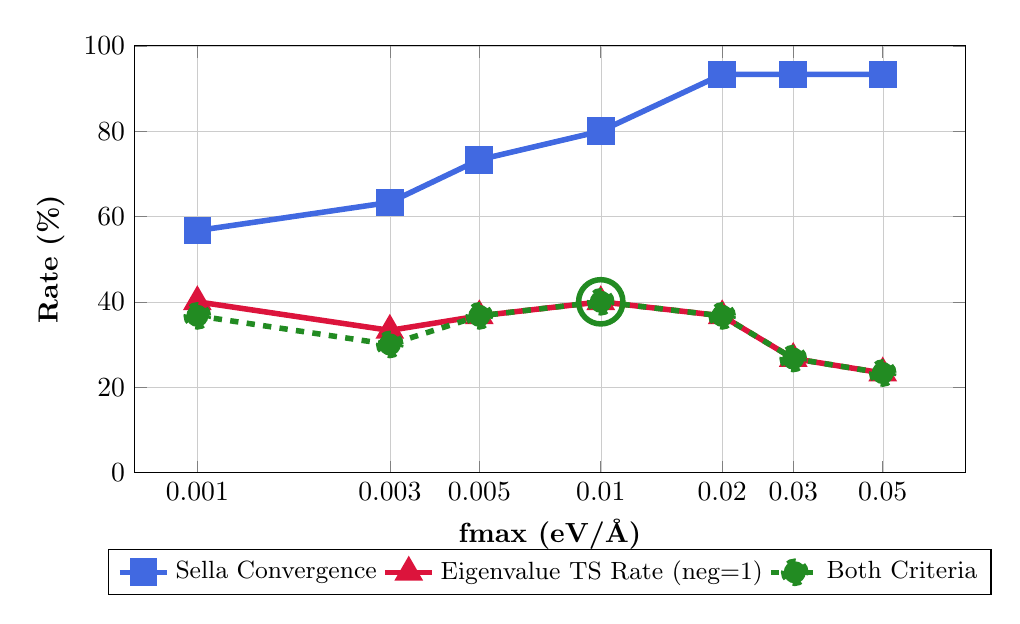
\begin{tikzpicture}
\begin{axis}[
    width=\textwidth,
    height=7cm,
    xlabel={\textbf{fmax (eV/\AA)}},
    ylabel={\textbf{Rate (\%)}},
    xmode=log,
    xmin=0.0007, xmax=0.08,
    ymin=0, ymax=100,
    xtick={0.001, 0.003, 0.005, 0.01, 0.02, 0.03, 0.05},
    xticklabels={0.001, 0.003, 0.005, 0.01, 0.02, 0.03, 0.05},
    legend style={at={(0.5,-0.18)}, anchor=north, legend columns=3, font=\small},
    grid=major,
    grid style={line width=0.1pt, draw=gray!40},
]

\addplot[color=sellaconv, mark=square*, mark size=4pt, line width=2pt] coordinates {
    (0.001, 56.7) (0.003, 63.3) (0.005, 73.3) (0.01, 80.0) (0.02, 93.3) (0.03, 93.3) (0.05, 93.3)
};
\addlegendentry{Sella Convergence}

\addplot[color=tsrate, mark=triangle*, mark size=4pt, line width=2pt] coordinates {
    (0.001, 40.0) (0.003, 33.3) (0.005, 36.7) (0.01, 40.0) (0.02, 36.7) (0.03, 26.7) (0.05, 23.3)
};
\addlegendentry{Eigenvalue TS Rate (neg=1)}

\addplot[color=bothrate, mark=*, mark size=4pt, line width=2pt, dashed] coordinates {
    (0.001, 36.7) (0.003, 30.0) (0.005, 36.7) (0.01, 40.0) (0.02, 36.7) (0.03, 26.7) (0.05, 23.3)
};
\addlegendentry{Both Criteria}

% Optimal marker
\draw[bothrate, line width=2pt] (axis cs:0.01, 40.0) circle (8pt);

\end{axis}
\end{tikzpicture}
\end{figure}

% ============================================================================
% STEPS BAR CHART
% ============================================================================
\section*{Computational Cost}

\begin{figure}[h!]
\centering
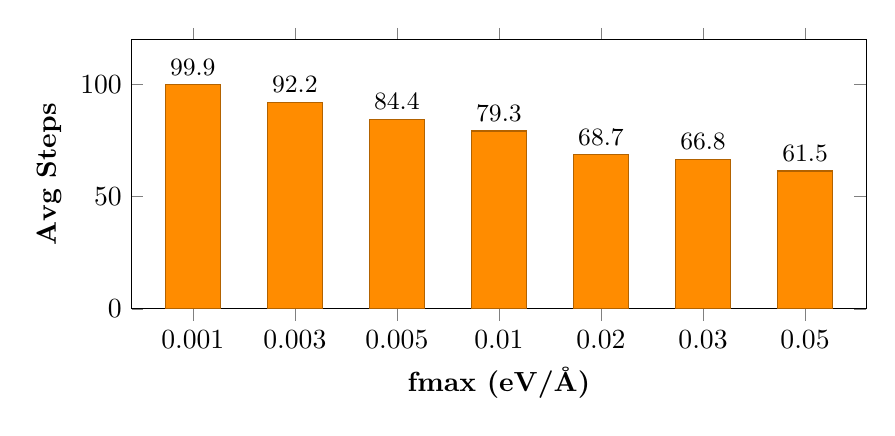
\begin{tikzpicture}
\begin{axis}[
    width=0.9\textwidth,
    height=5cm,
    xlabel={\textbf{fmax (eV/\AA)}},
    ylabel={\textbf{Avg Steps}},
    symbolic x coords={0.001, 0.003, 0.005, 0.01, 0.02, 0.03, 0.05},
    xtick=data,
    ymin=0, ymax=120,
    ybar,
    bar width=20pt,
    nodes near coords,
    nodes near coords align={vertical},
    every node near coord/.append style={font=\small\bfseries},
]
\addplot[fill=avgsteps, draw=avgsteps!70!black] coordinates {
    (0.001, 99.9) (0.003, 92.2) (0.005, 84.4) (0.01, 79.3) (0.02, 68.7) (0.03, 66.8) (0.05, 61.5)
};
\end{axis}
\end{tikzpicture}
\end{figure}

% ============================================================================
% TRADE-OFF SCATTER
% ============================================================================
\section*{Sella Convergence vs.\ TS Rate Trade-off}

\begin{figure}[h!]
\centering
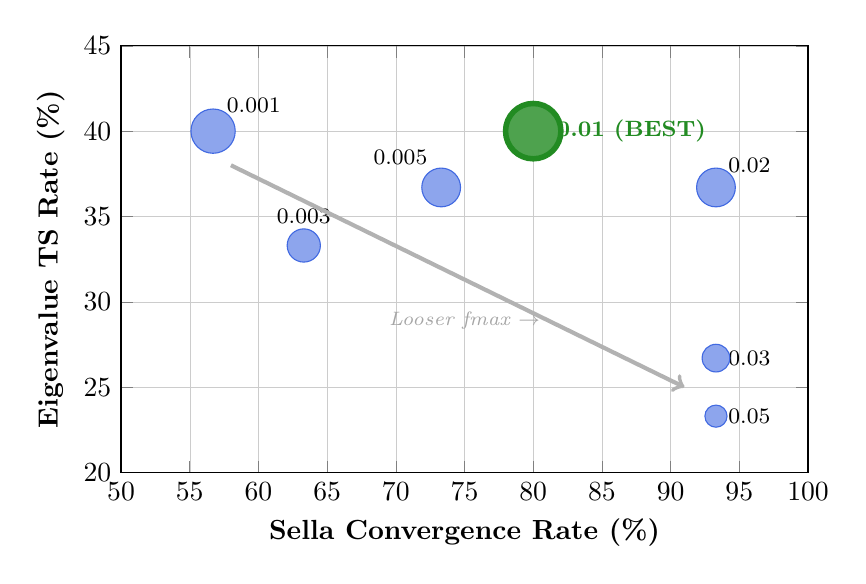
\begin{tikzpicture}
\begin{axis}[
    width=0.85\textwidth,
    height=7cm,
    xlabel={\textbf{Sella Convergence Rate (\%)}},
    ylabel={\textbf{Eigenvalue TS Rate (\%)}},
    xmin=50, xmax=100,
    ymin=20, ymax=45,
    grid=major,
    grid style={line width=0.1pt, draw=gray!40},
]

% Points with size proportional to "Both" rate
\addplot[only marks, mark=*, mark size=8pt, fill=sellaconv!60, draw=sellaconv] coordinates {(56.7, 40.0)};
\addplot[only marks, mark=*, mark size=6pt, fill=sellaconv!60, draw=sellaconv] coordinates {(63.3, 33.3)};
\addplot[only marks, mark=*, mark size=7pt, fill=sellaconv!60, draw=sellaconv] coordinates {(73.3, 36.7)};
\addplot[only marks, mark=*, mark size=10pt, fill=bothrate!80, draw=bothrate, line width=2pt] coordinates {(80.0, 40.0)};
\addplot[only marks, mark=*, mark size=7pt, fill=sellaconv!60, draw=sellaconv] coordinates {(93.3, 36.7)};
\addplot[only marks, mark=*, mark size=5pt, fill=sellaconv!60, draw=sellaconv] coordinates {(93.3, 26.7)};
\addplot[only marks, mark=*, mark size=4pt, fill=sellaconv!60, draw=sellaconv] coordinates {(93.3, 23.3)};

% Labels
\node[anchor=south west, font=\footnotesize] at (axis cs:57, 40.5) {0.001};
\node[anchor=south, font=\footnotesize] at (axis cs:63.3, 34) {0.003};
\node[anchor=south east, font=\footnotesize] at (axis cs:73, 37.5) {0.005};
\node[anchor=west, font=\footnotesize\bfseries, color=bothrate] at (axis cs:81, 40) {0.01 (BEST)};
\node[anchor=south west, font=\footnotesize] at (axis cs:93.5, 37) {0.02};
\node[anchor=west, font=\footnotesize] at (axis cs:93.5, 26.7) {0.03};
\node[anchor=west, font=\footnotesize] at (axis cs:93.5, 23.3) {0.05};

% Trend arrow
\draw[->, line width=1.5pt, gray!60] (axis cs:58, 38) -- (axis cs:91, 25);
\node[anchor=north, font=\scriptsize\itshape, gray!70] at (axis cs:75, 30) {Looser fmax $\rightarrow$};

\end{axis}
\end{tikzpicture}
\caption*{Point size $\propto$ Both criteria rate. Optimal at fmax=0.01.}
\end{figure}

% ============================================================================
% STACKED BAR: CONVERGENCE BREAKDOWN
% ============================================================================
\section*{Convergence Breakdown by fmax}

\begin{figure}[h!]
\centering
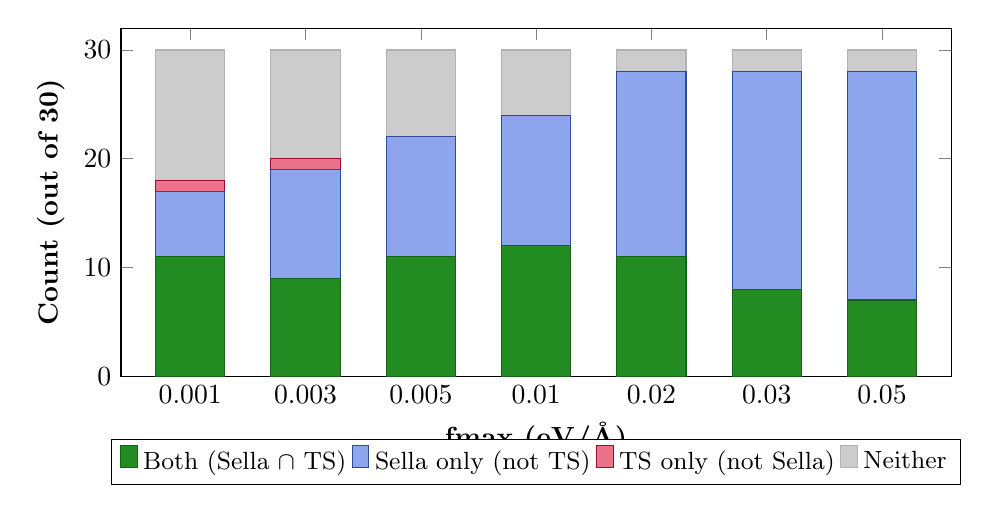
\begin{tikzpicture}
\begin{axis}[
    width=\textwidth,
    height=6cm,
    ybar stacked,
    bar width=25pt,
    symbolic x coords={0.001, 0.003, 0.005, 0.01, 0.02, 0.03, 0.05},
    xtick=data,
    xlabel={\textbf{fmax (eV/\AA)}},
    ylabel={\textbf{Count (out of 30)}},
    ymin=0, ymax=32,
    legend style={at={(0.5,-0.18)}, anchor=north, legend columns=4, font=\small},
    enlarge x limits=0.1,
]

% Both (Sella + TS) - bottom
\addplot[fill=bothrate, draw=bothrate!70!black] coordinates {
    (0.001, 11) (0.003, 9) (0.005, 11) (0.01, 12) (0.02, 11) (0.03, 8) (0.05, 7)
};
\addlegendentry{Both (Sella $\cap$ TS)}

% Sella only (converged but not TS) 
\addplot[fill=sellaconv!60, draw=sellaconv!70!black] coordinates {
    (0.001, 6) (0.003, 10) (0.005, 11) (0.01, 12) (0.02, 17) (0.03, 20) (0.05, 21)
};
\addlegendentry{Sella only (not TS)}

% TS only (not converged but is TS) - should be 0 or 1 based on data
\addplot[fill=tsrate!60, draw=tsrate!70!black] coordinates {
    (0.001, 1) (0.003, 1) (0.005, 0) (0.01, 0) (0.02, 0) (0.03, 0) (0.05, 0)
};
\addlegendentry{TS only (not Sella)}

% Neither
\addplot[fill=gray!40, draw=gray!60] coordinates {
    (0.001, 12) (0.003, 10) (0.005, 8) (0.01, 6) (0.02, 2) (0.03, 2) (0.05, 2)
};
\addlegendentry{Neither}

\end{axis}
\end{tikzpicture}
\end{figure}

% ============================================================================
% NEGATIVE EIGENVALUE DISTRIBUTION - ACTUAL DATA
% ============================================================================
\section*{Negative Eigenvalue Distribution by fmax}

\textbf{Key Finding:} No samples converged to minima (neg=0). All final structures have $\geq$1 negative eigenvalues.
Only 23--40\% are true TS (neg=1); the rest are higher-order saddles.

\begin{table}[h!]
\centering
\renewcommand{\arraystretch}{1.3}
\begin{tabular}{@{}r|>{\columncolor{neg1!20}}c|cccccc|c@{}}
\toprule
\textbf{fmax} & \textbf{neg=1} & \textbf{neg=2} & \textbf{neg=3} & \textbf{neg=4} & \textbf{neg=5} & \textbf{neg=6} & \textbf{neg=7} & \textbf{Total} \\
 & \textbf{(TS)} & & & & & & & \\
\midrule
0.001 & \textbf{12} & 9 & 4 & 2 & 1 & 2 & 0 & 30 \\
0.003 & 10 & 8 & 7 & 3 & 1 & 1 & 0 & 30 \\
0.005 & 11 & 9 & 5 & 2 & 2 & 1 & 0 & 30 \\
\rowcolor{green!10} 0.01  & \textbf{12} & 8 & 5 & 2 & 1 & 2 & 0 & 30 \\
0.02  & 11 & 9 & 3 & 2 & 2 & 2 & 1 & 30 \\
0.03  & 8 & 8 & 7 & 2 & 2 & 2 & 1 & 30 \\
0.05  & 7 & 6 & 8 & 3 & 3 & 2 & 1 & 30 \\
\bottomrule
\end{tabular}
\caption{Complete negative eigenvalue distribution. TS (neg=1) column highlighted.}
\end{table}

% Stacked bar with real data
\begin{figure}[h!]
\centering
\begin{tikzpicture}
\begin{axis}[
    width=\textwidth,
    height=7cm,
    ybar stacked,
    bar width=25pt,
    symbolic x coords={0.001, 0.003, 0.005, 0.01, 0.02, 0.03, 0.05},
    xtick=data,
    xlabel={\textbf{fmax (eV/\AA)}},
    ylabel={\textbf{Count (out of 30)}},
    ymin=0, ymax=32,
    legend style={at={(0.5,-0.15)}, anchor=north, legend columns=4, font=\small},
    enlarge x limits=0.1,
]

% neg=1 (TS) - BOTTOM so it's most visible
\addplot[fill=neg1, draw=neg1!70!black] coordinates {
    (0.001, 12) (0.003, 10) (0.005, 11) (0.01, 12) (0.02, 11) (0.03, 8) (0.05, 7)
};
\addlegendentry{neg=1 (TS) \checkmark}

% neg=2
\addplot[fill=neg2, draw=neg2!70!black] coordinates {
    (0.001, 9) (0.003, 8) (0.005, 9) (0.01, 8) (0.02, 9) (0.03, 8) (0.05, 6)
};
\addlegendentry{neg=2}

% neg=3
\addplot[fill=neg3, draw=neg3!70!black] coordinates {
    (0.001, 4) (0.003, 7) (0.005, 5) (0.01, 5) (0.02, 3) (0.03, 7) (0.05, 8)
};
\addlegendentry{neg=3}

% neg=4+
\addplot[fill=negmore, draw=negmore!70!black] coordinates {
    (0.001, 5) (0.003, 5) (0.005, 5) (0.01, 5) (0.02, 7) (0.03, 7) (0.05, 9)
};
\addlegendentry{neg$\geq$4}

\end{axis}
\end{tikzpicture}
\caption{Stacked distribution of negative eigenvalues. Blue (bottom) = true TS.}
\end{figure}

% Grouped bar comparison
\begin{figure}[h!]
\centering
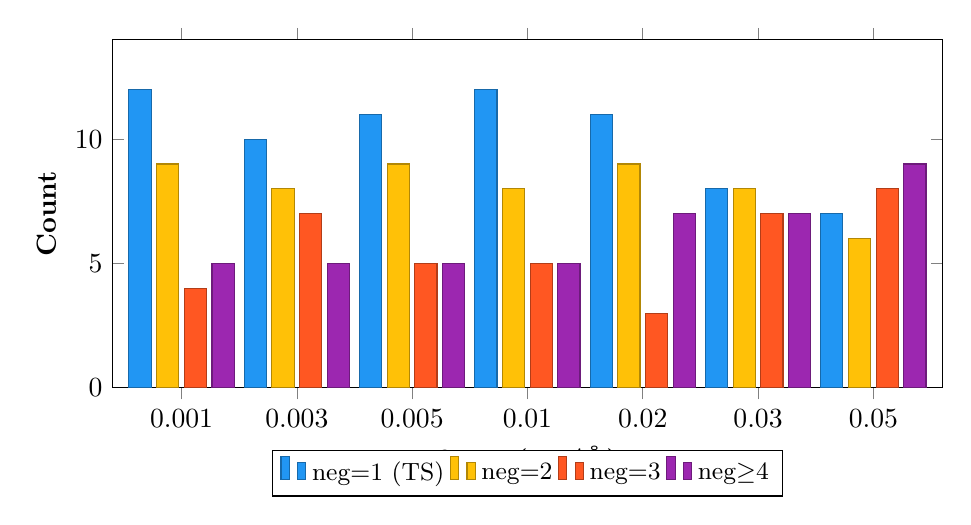
\begin{tikzpicture}
\begin{axis}[
    width=\textwidth,
    height=6cm,
    ybar,
    bar width=8pt,
    symbolic x coords={0.001, 0.003, 0.005, 0.01, 0.02, 0.03, 0.05},
    xtick=data,
    xlabel={\textbf{fmax (eV/\AA)}},
    ylabel={\textbf{Count}},
    ymin=0, ymax=14,
    legend style={at={(0.5,-0.18)}, anchor=north, legend columns=4, font=\small},
    enlarge x limits=0.1,
]

% neg=1
\addplot[fill=neg1, draw=neg1!70!black] coordinates {
    (0.001, 12) (0.003, 10) (0.005, 11) (0.01, 12) (0.02, 11) (0.03, 8) (0.05, 7)
};
\addlegendentry{neg=1 (TS)}

% neg=2
\addplot[fill=neg2, draw=neg2!70!black] coordinates {
    (0.001, 9) (0.003, 8) (0.005, 9) (0.01, 8) (0.02, 9) (0.03, 8) (0.05, 6)
};
\addlegendentry{neg=2}

% neg=3
\addplot[fill=neg3, draw=neg3!70!black] coordinates {
    (0.001, 4) (0.003, 7) (0.005, 5) (0.01, 5) (0.02, 3) (0.03, 7) (0.05, 8)
};
\addlegendentry{neg=3}

% neg>=4
\addplot[fill=negmore, draw=negmore!70!black] coordinates {
    (0.001, 5) (0.003, 5) (0.005, 5) (0.01, 5) (0.02, 7) (0.03, 7) (0.05, 9)
};
\addlegendentry{neg$\geq$4}

\end{axis}
\end{tikzpicture}
\caption{Grouped bar comparison showing shift toward higher-order saddles with looser fmax.}
\end{figure}

% TS vs non-TS pie-style comparison
\begin{figure}[h!]
\centering
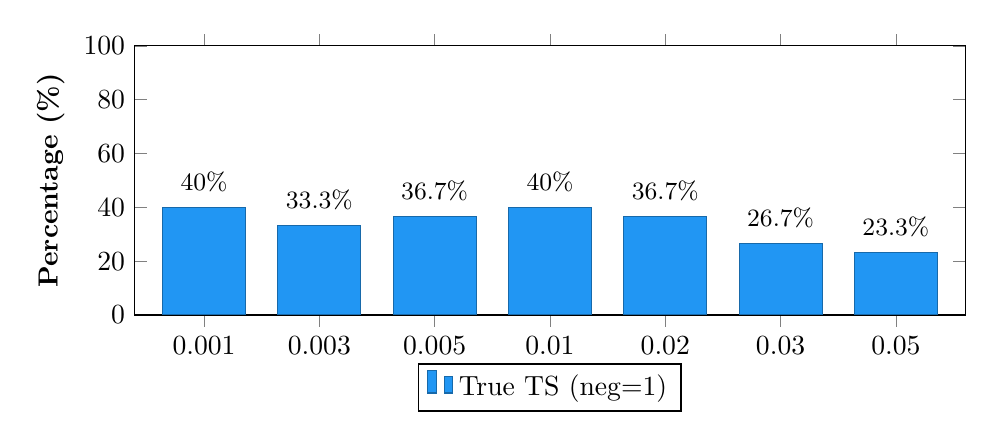
\begin{tikzpicture}
\begin{axis}[
    width=\textwidth,
    height=5cm,
    ybar,
    bar width=30pt,
    symbolic x coords={0.001, 0.003, 0.005, 0.01, 0.02, 0.03, 0.05},
    xtick=data,
    xlabel={\textbf{fmax (eV/\AA)}},
    ylabel={\textbf{Percentage (\%)}},
    ymin=0, ymax=100,
    legend style={at={(0.5,-0.18)}, anchor=north, legend columns=2, font=\normalsize},
    enlarge x limits=0.1,
    nodes near coords={\pgfmathprintnumber{\pgfplotspointmeta}\%},
    every node near coord/.append style={font=\small, yshift=2pt},
]

% TS rate
\addplot[fill=neg1, draw=neg1!70!black] coordinates {
    (0.001, 40) (0.003, 33.3) (0.005, 36.7) (0.01, 40) (0.02, 36.7) (0.03, 26.7) (0.05, 23.3)
};
\addlegendentry{True TS (neg=1)}

\end{axis}
\end{tikzpicture}
\caption{Percentage of true transition states (exactly 1 negative eigenvalue) by fmax.}
\end{figure}

% ============================================================================
% NUMERICAL SUMMARY
% ============================================================================
\section*{Complete Numerical Summary}

\begin{table}[h!]
\centering
\renewcommand{\arraystretch}{1.3}
\small
\begin{tabular}{@{}l|ccccccc@{}}
\toprule
\textbf{fmax (eV/\AA)} & \textbf{0.001} & \textbf{0.003} & \textbf{0.005} & \cellcolor{green!15}\textbf{0.01} & \textbf{0.02} & \textbf{0.03} & \textbf{0.05} \\
\midrule
\multicolumn{8}{l}{\textit{Convergence Counts (out of 30):}} \\
\quad Sella converged & 17 & 19 & 22 & \cellcolor{green!15}24 & 28 & 28 & 28 \\
\quad TS (neg=1) & 12 & 10 & 11 & \cellcolor{green!15}12 & 11 & 8 & 7 \\
\quad Both criteria & 11 & 9 & 11 & \cellcolor{green!15}\textbf{12} & 11 & 8 & 7 \\
\quad Sella only & 6 & 10 & 11 & 12 & 17 & 20 & 21 \\
\quad TS only & 1 & 1 & 0 & 0 & 0 & 0 & 0 \\
\quad Neither & 12 & 10 & 8 & 6 & 2 & 2 & 2 \\
\midrule
\multicolumn{8}{l}{\textit{Eigenvalue Distribution (counts):}} \\
\quad neg=1 (TS) & 12 & 10 & 11 & \cellcolor{green!15}12 & 11 & 8 & 7 \\
\quad neg=2 & 9 & 8 & 9 & 8 & 9 & 8 & 6 \\
\quad neg=3 & 4 & 7 & 5 & 5 & 3 & 7 & 8 \\
\quad neg=4 & 2 & 3 & 2 & 2 & 2 & 2 & 3 \\
\quad neg=5 & 1 & 1 & 2 & 1 & 2 & 2 & 3 \\
\quad neg=6 & 2 & 1 & 1 & 2 & 2 & 2 & 2 \\
\quad neg=7 & 0 & 0 & 0 & 0 & 1 & 1 & 1 \\
\midrule
\multicolumn{8}{l}{\textit{Summary Statistics:}} \\
\quad neg$\geq$2 (not TS) & 18 & 20 & 19 & 18 & 19 & 22 & 23 \\
\quad neg$\geq$4 (high order) & 5 & 5 & 5 & 5 & 7 & 7 & 9 \\
\midrule
\multicolumn{8}{l}{\textit{Rates (\%):}} \\
\quad Sella rate & 56.7 & 63.3 & 73.3 & \cellcolor{green!15}80.0 & 93.3 & 93.3 & 93.3 \\
\quad TS rate & 40.0 & 33.3 & 36.7 & \cellcolor{green!15}40.0 & 36.7 & 26.7 & 23.3 \\
\quad Both rate & 36.7 & 30.0 & 36.7 & \cellcolor{green!15}\textbf{40.0} & 36.7 & 26.7 & 23.3 \\
\midrule
\multicolumn{8}{l}{\textit{Computational Cost:}} \\
\quad Avg steps & 99.9 & 92.2 & 84.4 & \cellcolor{green!15}79.3 & 68.7 & 66.8 & 61.5 \\
\bottomrule
\end{tabular}
\caption{Complete numerical results. Green = optimal (fmax=0.01). Note: 0\% converged to minima (neg=0).}
\end{table}

% ============================================================================
% BEST CONFIG BOX
% ============================================================================
\vspace{1em}
\noindent\fbox{\parbox{0.97\textwidth}{
\centering\large\textbf{OPTIMAL: fmax = 0.01 eV/\AA}\\[0.5em]
\normalsize
\begin{tabular}{lcl}
Sella convergence: & \textbf{80\%} & (24/30) \\
Eigenvalue TS rate: & \textbf{40\%} & (12/30) \\
Both criteria: & \textbf{40\%} & (12/30) \\
Average steps: & \textbf{79.3} & \\
\end{tabular}
}}

\end{document}
